\section{Algoritma Block Cipher Lainnya}
\label{sec:cipher-lainnya}

Selain DES, AES, GOST, dan RC, ada sejumlah \textit{block cipher} lain yang penting untuk
dikenal. Sebagian besar di antaranya ikut serta dalam kompetisi AES dan gagal, sebagian
lagi tetap dipakai karena sudah tertanam di sistem yang sulit diubah. Mempelajari
mereka bermanfaat bukan karena kita akan memakainya, melainkan karena setiap algoritma
memperlihatkan pilihan rancangan yang berbeda untuk masalah yang sama.

\subsection{Blowfish dan Twofish}

\textbf{Blowfish} dirancang oleh Bruce Schneier pada 1993 dan diterbitkan pada 1994
sebagai alternatif bebas paten bagi DES \citep{schneier1994blowfish}. Parameternya
adalah blok 64 bit, kunci 32 sampai 448 bit, dan 16 putaran dengan struktur Jaringan
Feistel.

Blowfish tidak memakai kotak-S yang tetap. Ia memiliki larik kunci putaran
$P[0..17]$ yang berisi delapan belas kata 32 bit, dan empat kotak-S
$S_1, S_2, S_3, S_4$ yang masing-masing berisi 256 entri 32 bit. Seluruhnya, yaitu
$18 + 4 \times 256 = 1042$ kata, dibangkitkan pada saat kunci dipasang, melalui prosedur
berikut:

\begin{enumerate}
    \item Isi larik $P$ dan keempat kotak-S dengan digit heksadesimal bilangan $\pi$.
          Digit $\pi$ dipakai sebagai sumber keacakan awal karena maknanya sudah
          diketahui publik, sehingga perancang tidak dapat menyembunyikan pilihan
          tertentu di dalamnya.
    \item XOR-kan $P[0]$ dengan 32 bit pertama kunci, $P[1]$ dengan 32 bit berikutnya,
          dan seterusnya secara bergilir sampai seluruh larik $P$ terpakai.
    \item Enkripsi blok nol dengan larik $P$ dan kotak-S yang sedang berlaku, lalu
          simpan kedua kata hasilnya sebagai $P[0]$ dan $P[1]$.
    \item Enkripsi blok nol lagi dengan larik yang baru saja diperbarui, lalu simpan
          hasilnya sebagai $P[2]$ dan $P[3]$. Ulangi sampai seluruh 18 entri $P$
          terisi.
    \item Lanjutkan prosedur yang sama untuk mengisi keempat kotak-S secara berurutan.
          Karena setiap enkripsi menghasilkan dua kata, diperlukan
          $1042/2 = 521$ enkripsi untuk menuntaskan seluruh proses.
\end{enumerate}

Prosedur ini menjelaskan mengapa Blowfish relatif lambat ketika kunci dipasang tetapi
sangat cepat ketika blok demi blok dienkripsi: seluruh biaya komputasi berada di depan.
Prosedur itu pula yang membuat Blowfish sangat tahan terhadap kriptanalisis yang
mengandalkan struktur kotak-S, sebab penyerang tidak pernah mengetahui isi keempat
kotak-S sebelum kuncinya ditebak.

Fungsi $F$ pada Blowfish menerima 32 bit dan memecahnya menjadi empat byte $a$, $b$,
$c$, dan $d$. Keempat byte itu dipakai sebagai indeks keempat kotak-S, lalu hasilnya
digabung dengan dua jenis operasi yang berbeda:

\begin{equation}
F(x) = \bigl( (S_1[a] \boxplus S_2[b]) \oplus S_3[c] \bigr) \boxplus S_4[d],
\label{eq:fungsi-f-blowfish}
\end{equation}

dengan $x = a \| b \| c \| d$ dan $\boxplus$ menyatakan penjumlahan modulo $2^{32}$.
Rangkaian operasi tersebut digambarkan pada Gambar~\ref{fig:fungsi-f-blowfish}.
Penggunaan penjumlahan dan XOR secara berselang-seling bukan kebetulan: XOR bersifat
linear atas bit sehingga mudah dianalisis, sedangkan penjumlahan memiliki penjalaran
bawaan (\textit{carry}) yang nonlinear. Menggabungkan keduanya memaksa penyerang
memperhitungkan dua aljabar yang berbeda sekaligus.

% Diagram fungsi F pada Blowfish.
% Dirujuk dari section-03.tex dengan % Diagram fungsi F pada Blowfish.
% Dirujuk dari section-03.tex dengan % Diagram fungsi F pada Blowfish.
% Dirujuk dari section-03.tex dengan \input{figures/fungsi-f-blowfish}.
\begin{figure}[htbp]
    \centering
    \begin{tikzpicture}[
        kotak/.style={draw, rounded corners=1pt, minimum height=0.85cm,
                      text width=2.2cm, align=center, font=\small, inner sep=2pt},
        op/.style={font=\small},
        panah/.style={-{Latex[length=2mm]}, thick},
        catatan/.style={font=\footnotesize, align=left, text width=12.6cm},
    ]
        \node[kotak] (s1) at (0,0)    {$S_1[a]$};
        \node[kotak] (s2) at (3.0,0)  {$S_2[b]$};
        \node[kotak] (s3) at (6.0,0)  {$S_3[c]$};
        \node[kotak] (s4) at (9.0,0)  {$S_4[d]$};
        \node[op] (o1) at (1.5,0)  {$+$};
        \node[op] (o2) at (4.5,0)  {$\oplus$};
        \node[op] (o3) at (7.5,0)  {$+$};
        \node (f)  at (11.3,0)  {$F(x)$};

        \draw[panah] (s1) -- (o1);
        \draw[panah] (o1) -- (s2);
        \draw[panah] (s2) -- (o2);
        \draw[panah] (o2) -- (s3);
        \draw[panah] (s3) -- (o3);
        \draw[panah] (o3) -- (s4);
        \draw[panah] (s4) -- (f);

        \node[font=\footnotesize, anchor=north] at (1.5,-0.62) {$\bmod 2^{32}$};
        \node[font=\footnotesize, anchor=north] at (7.5,-0.62) {$\bmod 2^{32}$};

        \node[font=\footnotesize, anchor=south] at (0,-0.12)  {$a$};
        \node[font=\footnotesize, anchor=south] at (3.0,-0.12) {$b$};
        \node[font=\footnotesize, anchor=south] at (6.0,-0.12) {$c$};
        \node[font=\footnotesize, anchor=south] at (9.0,-0.12) {$d$};

        \node[catatan, anchor=north] at (5.1,-1.25)
            {$x$ (32 bit) dipecah menjadi empat byte $a, b, c, d$. Setiap kotak-S
             berisi 256 entri 32 bit dan seluruhnya dibangkitkan dari kunci, sehingga
             penyerang tidak pernah mengetahuinya sebelum kunci ditebak};
    \end{tikzpicture}
    \caption{Fungsi $F$ pada Blowfish. Dua penjumlahan modulo $2^{32}$ dipisahkan oleh
    satu XOR, sehingga luaran tidak dapat dipisahkan per byte}
    \label{fig:fungsi-f-blowfish}
    \sumber{Munir, \textit{IF4020 Kriptografi}, ITB; Schneier, \textit{Blowfish}.}
\end{figure}
.
\begin{figure}[htbp]
    \centering
    \begin{tikzpicture}[
        kotak/.style={draw, rounded corners=1pt, minimum height=0.85cm,
                      text width=2.2cm, align=center, font=\small, inner sep=2pt},
        op/.style={font=\small},
        panah/.style={-{Latex[length=2mm]}, thick},
        catatan/.style={font=\footnotesize, align=left, text width=12.6cm},
    ]
        \node[kotak] (s1) at (0,0)    {$S_1[a]$};
        \node[kotak] (s2) at (3.0,0)  {$S_2[b]$};
        \node[kotak] (s3) at (6.0,0)  {$S_3[c]$};
        \node[kotak] (s4) at (9.0,0)  {$S_4[d]$};
        \node[op] (o1) at (1.5,0)  {$+$};
        \node[op] (o2) at (4.5,0)  {$\oplus$};
        \node[op] (o3) at (7.5,0)  {$+$};
        \node (f)  at (11.3,0)  {$F(x)$};

        \draw[panah] (s1) -- (o1);
        \draw[panah] (o1) -- (s2);
        \draw[panah] (s2) -- (o2);
        \draw[panah] (o2) -- (s3);
        \draw[panah] (s3) -- (o3);
        \draw[panah] (o3) -- (s4);
        \draw[panah] (s4) -- (f);

        \node[font=\footnotesize, anchor=north] at (1.5,-0.62) {$\bmod 2^{32}$};
        \node[font=\footnotesize, anchor=north] at (7.5,-0.62) {$\bmod 2^{32}$};

        \node[font=\footnotesize, anchor=south] at (0,-0.12)  {$a$};
        \node[font=\footnotesize, anchor=south] at (3.0,-0.12) {$b$};
        \node[font=\footnotesize, anchor=south] at (6.0,-0.12) {$c$};
        \node[font=\footnotesize, anchor=south] at (9.0,-0.12) {$d$};

        \node[catatan, anchor=north] at (5.1,-1.25)
            {$x$ (32 bit) dipecah menjadi empat byte $a, b, c, d$. Setiap kotak-S
             berisi 256 entri 32 bit dan seluruhnya dibangkitkan dari kunci, sehingga
             penyerang tidak pernah mengetahuinya sebelum kunci ditebak};
    \end{tikzpicture}
    \caption{Fungsi $F$ pada Blowfish. Dua penjumlahan modulo $2^{32}$ dipisahkan oleh
    satu XOR, sehingga luaran tidak dapat dipisahkan per byte}
    \label{fig:fungsi-f-blowfish}
    \sumber{Munir, \textit{IF4020 Kriptografi}, ITB; Schneier, \textit{Blowfish}.}
\end{figure}
.
\begin{figure}[htbp]
    \centering
    \begin{tikzpicture}[
        kotak/.style={draw, rounded corners=1pt, minimum height=0.85cm,
                      text width=2.2cm, align=center, font=\small, inner sep=2pt},
        op/.style={font=\small},
        panah/.style={-{Latex[length=2mm]}, thick},
        catatan/.style={font=\footnotesize, align=left, text width=12.6cm},
    ]
        \node[kotak] (s1) at (0,0)    {$S_1[a]$};
        \node[kotak] (s2) at (3.0,0)  {$S_2[b]$};
        \node[kotak] (s3) at (6.0,0)  {$S_3[c]$};
        \node[kotak] (s4) at (9.0,0)  {$S_4[d]$};
        \node[op] (o1) at (1.5,0)  {$+$};
        \node[op] (o2) at (4.5,0)  {$\oplus$};
        \node[op] (o3) at (7.5,0)  {$+$};
        \node (f)  at (11.3,0)  {$F(x)$};

        \draw[panah] (s1) -- (o1);
        \draw[panah] (o1) -- (s2);
        \draw[panah] (s2) -- (o2);
        \draw[panah] (o2) -- (s3);
        \draw[panah] (s3) -- (o3);
        \draw[panah] (o3) -- (s4);
        \draw[panah] (s4) -- (f);

        \node[font=\footnotesize, anchor=north] at (1.5,-0.62) {$\bmod 2^{32}$};
        \node[font=\footnotesize, anchor=north] at (7.5,-0.62) {$\bmod 2^{32}$};

        \node[font=\footnotesize, anchor=south] at (0,-0.12)  {$a$};
        \node[font=\footnotesize, anchor=south] at (3.0,-0.12) {$b$};
        \node[font=\footnotesize, anchor=south] at (6.0,-0.12) {$c$};
        \node[font=\footnotesize, anchor=south] at (9.0,-0.12) {$d$};

        \node[catatan, anchor=north] at (5.1,-1.25)
            {$x$ (32 bit) dipecah menjadi empat byte $a, b, c, d$. Setiap kotak-S
             berisi 256 entri 32 bit dan seluruhnya dibangkitkan dari kunci, sehingga
             penyerang tidak pernah mengetahuinya sebelum kunci ditebak};
    \end{tikzpicture}
    \caption{Fungsi $F$ pada Blowfish. Dua penjumlahan modulo $2^{32}$ dipisahkan oleh
    satu XOR, sehingga luaran tidak dapat dipisahkan per byte}
    \label{fig:fungsi-f-blowfish}
    \sumber{Munir, \textit{IF4020 Kriptografi}, ITB; Schneier, \textit{Blowfish}.}
\end{figure}


Enkripsi Blowfish mengikuti pola Feistel 16 putaran. Pada setiap putaran ke-$i$,
setengah blok kiri di-XOR dengan kunci putaran $P[i-1]$, fungsi $F$ dikenakan atas hasil
XOR dengan kunci putaran $P[i]$ pada setengah blok kanan dan hasilnya di-XOR dengan
setengah blok kiri, lalu kedua setengah blok bertukar peran. Setelah 16 putaran,
pertukaran terakhir dibatalkan dan enkripsi ditutup dengan penyaringan
$R \leftarrow R \oplus P[17]$, $L \leftarrow L \oplus P[18]$ dengan penomoran satu-basis
seperti pada bahan sumber. Penyaringan di kedua ujung inilah yang membuat dua blok
plainteks yang hanya berbeda pada putaran pertama tetap menghasilkan cipherteks yang
sama sekali berbeda.

Dua catatan praktis perlu disampaikan. Pertama, Blowfish memiliki sejumlah kecil kunci
lemah yang dapat dikenali dari nilai larik $P$ hasil pembangkitan. Cara pencegahan yang
disarankan perancangnya sederhana: \textit{hash} kunci terlebih dahulu, misalnya dengan
SHA-256, sebelum diserahkan kepada Blowfish, sehingga kunci lemah tidak pernah tercapai.
Kedua, seperti halnya GOST, ukuran blok 64 bit membatasi banyaknya data yang boleh
dienkripsi dengan satu kunci sampai sekitar $2^{32}$ blok, yaitu sekitar 32 GiB.
Karena itu Blowfish tidak lagi dianjurkan untuk sistem baru; keberadaannya kini
dipertahankan terutama untuk menjaga kompatibilitas.

\textbf{Twofish} adalah kelanjutan Blowfish oleh Schneier bersama Kelsey, Whiting,
Wagner, Hall, dan Ferguson, dan merupakan salah satu dari lima finalis AES
\citep{schneier1998twofish}. Bloknya diperbesar menjadi 128 bit dan panjang kuncinya
128, 192, atau 256 bit, sedangkan jumlah putarannya 16. Meskipun masih berkerabat
dengan Blowfish, Twofish bukan Feistel murni: ia mengolah dua kata sekaligus dalam satu
putaran dan memakai penyaringan kunci di awal dan di akhir.

Inti Twofish adalah fungsi $g$ yang menyaring 32 bit masukan melalui empat kotak-S
$8 \times 8$ yang bergantung pada kunci, dilanjutkan dengan perkalian oleh sebuah
matriks MDS (\textit{maximum distance separable}) berukuran $4 \times 4$ atas medan
$\text{GF}(2^8)$, lalu digabungkan dengan luaran $g$ yang kedua melalui transformasi
PHT (\textit{pseudo-Hadamard transform}) berbentuk $(u, v) \mapsto (u + v,\ u + 2v)$
dengan seluruh penjumlahan modulo $2^{32}$. Rangkaian itu ditampilkan pada
Gambar~\ref{fig:fungsi-g-twofish}.

% Diagram fungsi g pada Twofish: empat kotak-S bergantung kunci, matriks MDS, lalu PHT.
% Dirujuk dari section-03.tex dengan % Diagram fungsi g pada Twofish: empat kotak-S bergantung kunci, matriks MDS, lalu PHT.
% Dirujuk dari section-03.tex dengan % Diagram fungsi g pada Twofish: empat kotak-S bergantung kunci, matriks MDS, lalu PHT.
% Dirujuk dari section-03.tex dengan \input{figures/fungsi-g-twofish}.
\begin{figure}[htbp]
    \centering
    \begin{tikzpicture}[
        kotak/.style={draw, rounded corners=1pt, minimum height=0.72cm,
                      text width=1.5cm, align=center, font=\small, inner sep=2pt},
        besar/.style={draw, rounded corners=1pt, minimum height=1.1cm,
                      text width=2.5cm, align=center, font=\small, inner sep=2pt},
        panah/.style={-{Latex[length=2mm]}, thick},
        catatan/.style={font=\footnotesize, align=left, text width=11.6cm},
    ]
        \node (x) at (0,0) {$X$};
        \node[kotak] (s0) at (2.4, 1.35) {$S_0[x_0]$};
        \node[kotak] (s1) at (2.4, 0.45) {$S_1[x_1]$};
        \node[kotak] (s2) at (2.4,-0.45) {$S_2[x_2]$};
        \node[kotak] (s3) at (2.4,-1.35) {$S_3[x_3]$};
        \node[besar] (mds) at (5.4,0) {matriks MDS\\$4 \times 4$ di $\text{GF}(2^8)$};
        \node (t) at (7.9,0) {$T$};
        \node[besar] (pht) at (10.4,0) {PHT\\$(u,v) \mapsto (u+v,\ u+2v)$};
        \node (f) at (12.6,0) {$(F_0, F_1)$};

        \draw[panah] (x) -- (s0);
        \draw[panah] (x) -- (s1);
        \draw[panah] (x) -- (s2);
        \draw[panah] (x) -- (s3);
        \draw[panah] (s0) -- (mds);
        \draw[panah] (s1) -- (mds);
        \draw[panah] (s2) -- (mds);
        \draw[panah] (s3) -- (mds);
        \draw[panah] (mds) -- (t);
        \draw[panah] (t) -- (pht);
        \draw[panah] (pht) -- (f);

        \node[catatan, anchor=north west] at (-1.0,-2.2)
            {Setiap $S_j$ adalah kotak-S $8 \times 8$ yang bergantung pada kunci, dan
             $x_0, \dots, x_3$ adalah empat byte penyusun $X$. PHT menggabungkan
             luaran $g$ ini dengan luaran $g$ yang kedua menjadi pasangan $F_0, F_1$};
    \end{tikzpicture}
    \caption{Fungsi $g$ pada Twofish beserta penggabung PHT. Matriks MDS menjamin
    perubahan satu bit masukan menyebar ke seluruh byte keluaran}
    \label{fig:fungsi-g-twofish}
    \sumber{Munir, \textit{IF4020 Kriptografi}, ITB; Schneier dkk., \textit{Twofish}.}
\end{figure}
.
\begin{figure}[htbp]
    \centering
    \begin{tikzpicture}[
        kotak/.style={draw, rounded corners=1pt, minimum height=0.72cm,
                      text width=1.5cm, align=center, font=\small, inner sep=2pt},
        besar/.style={draw, rounded corners=1pt, minimum height=1.1cm,
                      text width=2.5cm, align=center, font=\small, inner sep=2pt},
        panah/.style={-{Latex[length=2mm]}, thick},
        catatan/.style={font=\footnotesize, align=left, text width=11.6cm},
    ]
        \node (x) at (0,0) {$X$};
        \node[kotak] (s0) at (2.4, 1.35) {$S_0[x_0]$};
        \node[kotak] (s1) at (2.4, 0.45) {$S_1[x_1]$};
        \node[kotak] (s2) at (2.4,-0.45) {$S_2[x_2]$};
        \node[kotak] (s3) at (2.4,-1.35) {$S_3[x_3]$};
        \node[besar] (mds) at (5.4,0) {matriks MDS\\$4 \times 4$ di $\text{GF}(2^8)$};
        \node (t) at (7.9,0) {$T$};
        \node[besar] (pht) at (10.4,0) {PHT\\$(u,v) \mapsto (u+v,\ u+2v)$};
        \node (f) at (12.6,0) {$(F_0, F_1)$};

        \draw[panah] (x) -- (s0);
        \draw[panah] (x) -- (s1);
        \draw[panah] (x) -- (s2);
        \draw[panah] (x) -- (s3);
        \draw[panah] (s0) -- (mds);
        \draw[panah] (s1) -- (mds);
        \draw[panah] (s2) -- (mds);
        \draw[panah] (s3) -- (mds);
        \draw[panah] (mds) -- (t);
        \draw[panah] (t) -- (pht);
        \draw[panah] (pht) -- (f);

        \node[catatan, anchor=north west] at (-1.0,-2.2)
            {Setiap $S_j$ adalah kotak-S $8 \times 8$ yang bergantung pada kunci, dan
             $x_0, \dots, x_3$ adalah empat byte penyusun $X$. PHT menggabungkan
             luaran $g$ ini dengan luaran $g$ yang kedua menjadi pasangan $F_0, F_1$};
    \end{tikzpicture}
    \caption{Fungsi $g$ pada Twofish beserta penggabung PHT. Matriks MDS menjamin
    perubahan satu bit masukan menyebar ke seluruh byte keluaran}
    \label{fig:fungsi-g-twofish}
    \sumber{Munir, \textit{IF4020 Kriptografi}, ITB; Schneier dkk., \textit{Twofish}.}
\end{figure}
.
\begin{figure}[htbp]
    \centering
    \begin{tikzpicture}[
        kotak/.style={draw, rounded corners=1pt, minimum height=0.72cm,
                      text width=1.5cm, align=center, font=\small, inner sep=2pt},
        besar/.style={draw, rounded corners=1pt, minimum height=1.1cm,
                      text width=2.5cm, align=center, font=\small, inner sep=2pt},
        panah/.style={-{Latex[length=2mm]}, thick},
        catatan/.style={font=\footnotesize, align=left, text width=11.6cm},
    ]
        \node (x) at (0,0) {$X$};
        \node[kotak] (s0) at (2.4, 1.35) {$S_0[x_0]$};
        \node[kotak] (s1) at (2.4, 0.45) {$S_1[x_1]$};
        \node[kotak] (s2) at (2.4,-0.45) {$S_2[x_2]$};
        \node[kotak] (s3) at (2.4,-1.35) {$S_3[x_3]$};
        \node[besar] (mds) at (5.4,0) {matriks MDS\\$4 \times 4$ di $\text{GF}(2^8)$};
        \node (t) at (7.9,0) {$T$};
        \node[besar] (pht) at (10.4,0) {PHT\\$(u,v) \mapsto (u+v,\ u+2v)$};
        \node (f) at (12.6,0) {$(F_0, F_1)$};

        \draw[panah] (x) -- (s0);
        \draw[panah] (x) -- (s1);
        \draw[panah] (x) -- (s2);
        \draw[panah] (x) -- (s3);
        \draw[panah] (s0) -- (mds);
        \draw[panah] (s1) -- (mds);
        \draw[panah] (s2) -- (mds);
        \draw[panah] (s3) -- (mds);
        \draw[panah] (mds) -- (t);
        \draw[panah] (t) -- (pht);
        \draw[panah] (pht) -- (f);

        \node[catatan, anchor=north west] at (-1.0,-2.2)
            {Setiap $S_j$ adalah kotak-S $8 \times 8$ yang bergantung pada kunci, dan
             $x_0, \dots, x_3$ adalah empat byte penyusun $X$. PHT menggabungkan
             luaran $g$ ini dengan luaran $g$ yang kedua menjadi pasangan $F_0, F_1$};
    \end{tikzpicture}
    \caption{Fungsi $g$ pada Twofish beserta penggabung PHT. Matriks MDS menjamin
    perubahan satu bit masukan menyebar ke seluruh byte keluaran}
    \label{fig:fungsi-g-twofish}
    \sumber{Munir, \textit{IF4020 Kriptografi}, ITB; Schneier dkk., \textit{Twofish}.}
\end{figure}


Perlu dicatat bahwa bahan sumber menyebut Twofish memiliki lima kotak-S. Yang benar
adalah empat kotak-S $8 \times 8$ yang bergantung pada kunci, yang masing-masing
disusun dari dua permutasi tetap $q_0$ dan $q_1$ dengan menyisipkan bahan kunci.
Perbedaan ini penting, karena justru sifat \emph{bergantung kunci} itulah yang menjadi
ciri khas keluarga Blowfish--Twofish sekaligus menjadi kelemahan mereka di perangkat
keras: kotak-S yang berubah setiap kali kunci berganti tidak dapat ditanam sebagai
tabel tetap di dalam sirkuit.

Matriks MDS pada Gambar~\ref{fig:fungsi-g-twofish} memainkan peran yang sama dengan
lapisan MixColumns pada AES, yaitu menyebarkan perubahan satu byte ke seluruh empat
byte keluaran. Satu putaran Twofish secara lengkap, termasuk penyaringan masukan dan
keluaran, ditampilkan pada Gambar~\ref{fig:putaran-twofish}.

\begin{figure}[htbp]
    \centering
    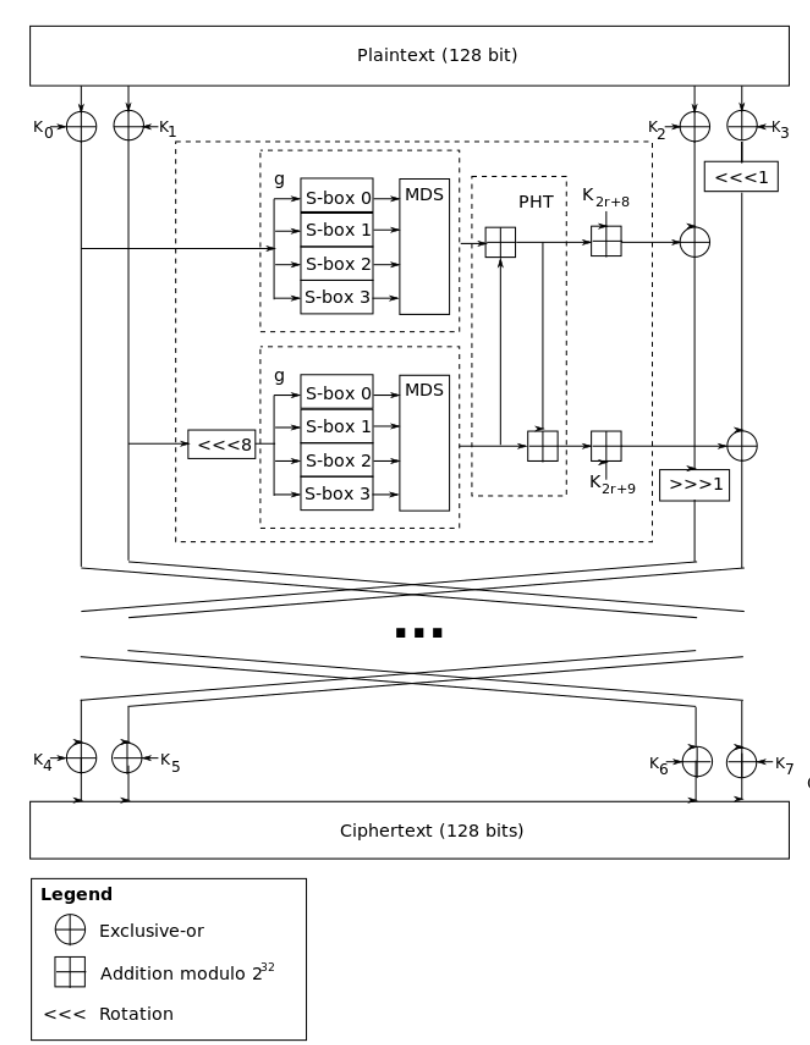
\includegraphics[width=0.9\linewidth, height=0.8\textheight, keepaspectratio]{figures/putaran-twofish.png}
    \caption{Rincian satu putaran algoritma Twofish: fungsi $g$ dengan empat S-box dan matriks MDS, transformasi PHT, rotasi bit, dan penambahan kunci putaran}
    \label{fig:putaran-twofish}
    \sumber{Munir, \textit{IF4020 Kriptografi}, ITB.}
\end{figure}

\subsection{Serpent dan MARS}

\textbf{Serpent} dirancang oleh Ross Anderson, Eli Biham, dan Lars Knudsen dan juga
merupakan finalis AES \citep{anderson1998serpent}. Bloknya 128 bit dengan kunci 128,
192, atau 256 bit, dan jumlah putarannya 32. Berbeda dari Blowfish dan Twofish,
Serpent sama sekali tidak memakai Jaringan Feistel: ia adalah jaringan
substitusi--permutasi (\textit{SPN}) murni, sebagaimana AES. Seluruh 128 bit diolah
sekaligus pada setiap putaran melalui tiga langkah yang berurutan: XOR dengan subkunci,
substitusi oleh 32 kotak-S yang bekerja serentak, dan transformasi linier. Strukturnya
ditampilkan pada Gambar~\ref{fig:putaran-serpent}.

% Diagram struktur putaran Serpent: 32 kali {XOR subkunci, kotak-S, transformasi linier}.
% Dirujuk dari section-03.tex dengan % Diagram struktur putaran Serpent: 32 kali {XOR subkunci, kotak-S, transformasi linier}.
% Dirujuk dari section-03.tex dengan % Diagram struktur putaran Serpent: 32 kali {XOR subkunci, kotak-S, transformasi linier}.
% Dirujuk dari section-03.tex dengan \input{figures/putaran-serpent}.
\begin{figure}[htbp]
    \centering
    \begin{tikzpicture}[
        kotak/.style={draw, rounded corners=1pt, minimum height=0.9cm,
                      text width=2.2cm, align=center, font=\small, inner sep=2pt},
        panah/.style={-{Latex[length=2mm]}, thick},
        catatan/.style={font=\footnotesize, align=left, text width=13.2cm},
    ]
        \node[kotak] (ip) at (0,0) {permutasi\\awal (IP)};
        \node[draw, rounded corners=1pt, inner sep=6pt,
              fit={(2.5,0.85) (9.5,-0.85)}] (rnd) {};
        \node[kotak] (kx)  at (3.0,0) {XOR dengan\\$\hat{K}_i$};
        \node[kotak] (sb)  at (5.5,0) {32 kotak-S\\$4 \times 4$ bit};
        \node[kotak] (lt)  at (8.0,0) {transformasi\\linier (LT)};
        \node[kotak] (ipv) at (11.4,0) {permutasi\\akhir (IP$^{-1}$)};

        \draw[panah] (ip) -- (rnd);
        \draw[panah] (kx) -- (sb);
        \draw[panah] (sb) -- (lt);
        \draw[panah] (rnd) -- (ipv);

        \node[font=\footnotesize, anchor=north] at (5.7,-1.1)
            {diulang 32 kali (putaran terakhir tanpa LT)};
        \node[catatan, anchor=north west] at (-1.0,-1.75)
            {Tiga puluh tiga subkunci $\hat{K}_0, \dots, \hat{K}_{32}$ diturunkan dari
             kunci melalui cipher itu sendiri, sehingga jadwal kuncinya justru lebih
             mahal daripada jadwal kunci DES};
    \end{tikzpicture}
    \caption{Struktur Serpent. Seluruh blok diproses dalam satu jalur substitusi-permutasi
    berputar, dengan sebuah transformasi linier bit demi bit sebagai pelebur antarputaran}
    \label{fig:putaran-serpent}
    \sumber{Munir, \textit{IF4020 Kriptografi}, ITB; Anderson, Biham, \& Knudsen, \textit{Serpent}.}
\end{figure}
.
\begin{figure}[htbp]
    \centering
    \begin{tikzpicture}[
        kotak/.style={draw, rounded corners=1pt, minimum height=0.9cm,
                      text width=2.2cm, align=center, font=\small, inner sep=2pt},
        panah/.style={-{Latex[length=2mm]}, thick},
        catatan/.style={font=\footnotesize, align=left, text width=13.2cm},
    ]
        \node[kotak] (ip) at (0,0) {permutasi\\awal (IP)};
        \node[draw, rounded corners=1pt, inner sep=6pt,
              fit={(2.5,0.85) (9.5,-0.85)}] (rnd) {};
        \node[kotak] (kx)  at (3.0,0) {XOR dengan\\$\hat{K}_i$};
        \node[kotak] (sb)  at (5.5,0) {32 kotak-S\\$4 \times 4$ bit};
        \node[kotak] (lt)  at (8.0,0) {transformasi\\linier (LT)};
        \node[kotak] (ipv) at (11.4,0) {permutasi\\akhir (IP$^{-1}$)};

        \draw[panah] (ip) -- (rnd);
        \draw[panah] (kx) -- (sb);
        \draw[panah] (sb) -- (lt);
        \draw[panah] (rnd) -- (ipv);

        \node[font=\footnotesize, anchor=north] at (5.7,-1.1)
            {diulang 32 kali (putaran terakhir tanpa LT)};
        \node[catatan, anchor=north west] at (-1.0,-1.75)
            {Tiga puluh tiga subkunci $\hat{K}_0, \dots, \hat{K}_{32}$ diturunkan dari
             kunci melalui cipher itu sendiri, sehingga jadwal kuncinya justru lebih
             mahal daripada jadwal kunci DES};
    \end{tikzpicture}
    \caption{Struktur Serpent. Seluruh blok diproses dalam satu jalur substitusi-permutasi
    berputar, dengan sebuah transformasi linier bit demi bit sebagai pelebur antarputaran}
    \label{fig:putaran-serpent}
    \sumber{Munir, \textit{IF4020 Kriptografi}, ITB; Anderson, Biham, \& Knudsen, \textit{Serpent}.}
\end{figure}
.
\begin{figure}[htbp]
    \centering
    \begin{tikzpicture}[
        kotak/.style={draw, rounded corners=1pt, minimum height=0.9cm,
                      text width=2.2cm, align=center, font=\small, inner sep=2pt},
        panah/.style={-{Latex[length=2mm]}, thick},
        catatan/.style={font=\footnotesize, align=left, text width=13.2cm},
    ]
        \node[kotak] (ip) at (0,0) {permutasi\\awal (IP)};
        \node[draw, rounded corners=1pt, inner sep=6pt,
              fit={(2.5,0.85) (9.5,-0.85)}] (rnd) {};
        \node[kotak] (kx)  at (3.0,0) {XOR dengan\\$\hat{K}_i$};
        \node[kotak] (sb)  at (5.5,0) {32 kotak-S\\$4 \times 4$ bit};
        \node[kotak] (lt)  at (8.0,0) {transformasi\\linier (LT)};
        \node[kotak] (ipv) at (11.4,0) {permutasi\\akhir (IP$^{-1}$)};

        \draw[panah] (ip) -- (rnd);
        \draw[panah] (kx) -- (sb);
        \draw[panah] (sb) -- (lt);
        \draw[panah] (rnd) -- (ipv);

        \node[font=\footnotesize, anchor=north] at (5.7,-1.1)
            {diulang 32 kali (putaran terakhir tanpa LT)};
        \node[catatan, anchor=north west] at (-1.0,-1.75)
            {Tiga puluh tiga subkunci $\hat{K}_0, \dots, \hat{K}_{32}$ diturunkan dari
             kunci melalui cipher itu sendiri, sehingga jadwal kuncinya justru lebih
             mahal daripada jadwal kunci DES};
    \end{tikzpicture}
    \caption{Struktur Serpent. Seluruh blok diproses dalam satu jalur substitusi-permutasi
    berputar, dengan sebuah transformasi linier bit demi bit sebagai pelebur antarputaran}
    \label{fig:putaran-serpent}
    \sumber{Munir, \textit{IF4020 Kriptografi}, ITB; Anderson, Biham, \& Knudsen, \textit{Serpent}.}
\end{figure}


Serpent memiliki delapan kotak-S berbeda, masing-masing berukuran $4 \times 4$ bit.
Pada setiap putaran, ke-32 nibble penyusun blok 128 bit disubstitusi secara serentak
dengan salah satu dari kedelapan kotak-S itu menurut pola yang tetap. Cara
implementasinya menarik: alih-alih menyimpan tabel, sebuah kata 32 bit dapat memuat 32
nibble yang berasal dari \emph{posisi} yang sama pada 32 blok berbeda. Teknik yang
dikenal sebagai \textit{bit-slicing} ini memungkinkan sebuah komputer 32 bit memproses
32 blok sekaligus dengan biaya satu blok, dan inilah alasan Serpent dirancang di sekitar
kotak-S $4 \times 4$ dan bukan kotak-S yang lebih besar.

Kekuatan Serpent terletak pada transformasi liniernya, yang dirancang memiliki
\textit{branch number} tinggi sehingga perbedaan satu bit pada masukan menyebar ke
beberapa bit sekaligus pada luaran. Akibatnya difusi tercapai jauh lebih cepat daripada
pada Feistel, dan 32 putaran menghasilkan margin keamanan yang sangat lebar: hingga
kini serangan terbaik yang dipublikasikan hanya mampu menjangkau sekitar sepertiga
dari seluruh putaran. Harga yang harus dibayar adalah kecepatan. Tanpa pemanfaatan
\textit{bit-slicing}, Serpent adalah finalis AES yang paling lambat di perangkat lunak;
inilah yang menjadi pertimbangan utama NIST ketika memilih Rijndael sebagai pemenang.

\textbf{MARS} diajukan oleh IBM dan merupakan finalis AES dengan perolehan suara
paling sedikit \citep{burwick1998mars}. Bloknya 128 bit dengan kunci 128 sampai 448 bit.
Yang membedakannya adalah struktur putarannya. Bahan sumber menyebut MARS melakukan
operasi substitusi--permutasi pada setiap putaran; gambaran itu kurang tepat. MARS
adalah Feistel tak seimbang (\textit{unbalanced Feistel}) dengan rancangan yang
heterogen, dan 32 putarannya terbagi menjadi tiga fase yang berbeda sifatnya
(Gambar~\ref{fig:mars-mixing}):

\begin{enumerate}
    \item \textbf{Delapan putaran \textit{forward mixing}} yang bekerja tanpa kunci.
          Fase ini memakai perkalian dan rotasi atas data untuk mempercepat
          penyebaran perubahan bit masukan.
    \item \textbf{Enam belas putaran inti} (\textit{core}) yang memakai kunci. Setiap
          putaran inti memakai pencarian kotak-S dan rotasi yang besarnya ditentukan
          oleh data itu sendiri.
    \item \textbf{Delapan putaran \textit{backward mixing}} yang juga bekerja tanpa
          kunci dan merupakan kebalikan dari fase pertama.
\end{enumerate}

% Diagram pembagian 32 putaran MARS: forward mixing, core, backward mixing.
% Dirujuk dari section-03.tex dengan % Diagram pembagian 32 putaran MARS: forward mixing, core, backward mixing.
% Dirujuk dari section-03.tex dengan % Diagram pembagian 32 putaran MARS: forward mixing, core, backward mixing.
% Dirujuk dari section-03.tex dengan \input{figures/mars-mixing}.
\begin{figure}[htbp]
    \centering
    \begin{tikzpicture}[
        fase/.style={draw, rounded corners=1pt, minimum height=1.3cm,
                     text width=3.9cm, align=center, font=\small, inner sep=3pt},
        panah/.style={-{Latex[length=2mm]}, thick},
        catatan/.style={font=\footnotesize, align=left, text width=12.9cm},
    ]
        \node[fase] (fwd) at (0,0)
            {\textbf{8 putaran}\\ \textit{forward mixing}\\
             perkalian, rotasi data,\\ penambahan kunci};
        \node[fase] (core) at (4.4,0)
            {\textbf{16 putaran}\\ \textit{core}\\
             kotak-S, rotasi bergantung\\ data, penambahan kunci};
        \node[fase] (bwd) at (8.8,0)
            {\textbf{8 putaran}\\ \textit{backward mixing}\\
             kebalikan \textit{forward mixing},\\ mengacak kembali};

        \draw[panah] (-2.2,0) -- (fwd);
        \draw[panah] (fwd) -- (core);
        \draw[panah] (core) -- (bwd);
        \draw[panah] (bwd) -- (11.0,0);

        \node[catatan, anchor=north] at (4.4,-1.4)
            {Kedua fase \textit{mixing} bekerja tanpa kunci dan dirancang agar tidak
             dapat dibalik. Seluruh 32 putaran memakai kunci hasil perluasan dari
             40 kata, sehingga biaya pemasangan kuncinya paling mahal di antara
             kelima finalis AES};
    \end{tikzpicture}
    \caption{Pembagian 32 putaran MARS. Rancangan ini menempatkan ketahanan terhadap
    kriptanalisis pada putaran inti, sementara putaran tepi mempercepat penyebaran
    perubahan bit masukan}
    \label{fig:mars-mixing}
    \sumber{Munir, \textit{IF4020 Kriptografi}, ITB; Burwick dkk., \textit{MARS}.}
\end{figure}
.
\begin{figure}[htbp]
    \centering
    \begin{tikzpicture}[
        fase/.style={draw, rounded corners=1pt, minimum height=1.3cm,
                     text width=3.9cm, align=center, font=\small, inner sep=3pt},
        panah/.style={-{Latex[length=2mm]}, thick},
        catatan/.style={font=\footnotesize, align=left, text width=12.9cm},
    ]
        \node[fase] (fwd) at (0,0)
            {\textbf{8 putaran}\\ \textit{forward mixing}\\
             perkalian, rotasi data,\\ penambahan kunci};
        \node[fase] (core) at (4.4,0)
            {\textbf{16 putaran}\\ \textit{core}\\
             kotak-S, rotasi bergantung\\ data, penambahan kunci};
        \node[fase] (bwd) at (8.8,0)
            {\textbf{8 putaran}\\ \textit{backward mixing}\\
             kebalikan \textit{forward mixing},\\ mengacak kembali};

        \draw[panah] (-2.2,0) -- (fwd);
        \draw[panah] (fwd) -- (core);
        \draw[panah] (core) -- (bwd);
        \draw[panah] (bwd) -- (11.0,0);

        \node[catatan, anchor=north] at (4.4,-1.4)
            {Kedua fase \textit{mixing} bekerja tanpa kunci dan dirancang agar tidak
             dapat dibalik. Seluruh 32 putaran memakai kunci hasil perluasan dari
             40 kata, sehingga biaya pemasangan kuncinya paling mahal di antara
             kelima finalis AES};
    \end{tikzpicture}
    \caption{Pembagian 32 putaran MARS. Rancangan ini menempatkan ketahanan terhadap
    kriptanalisis pada putaran inti, sementara putaran tepi mempercepat penyebaran
    perubahan bit masukan}
    \label{fig:mars-mixing}
    \sumber{Munir, \textit{IF4020 Kriptografi}, ITB; Burwick dkk., \textit{MARS}.}
\end{figure}
.
\begin{figure}[htbp]
    \centering
    \begin{tikzpicture}[
        fase/.style={draw, rounded corners=1pt, minimum height=1.3cm,
                     text width=3.9cm, align=center, font=\small, inner sep=3pt},
        panah/.style={-{Latex[length=2mm]}, thick},
        catatan/.style={font=\footnotesize, align=left, text width=12.9cm},
    ]
        \node[fase] (fwd) at (0,0)
            {\textbf{8 putaran}\\ \textit{forward mixing}\\
             perkalian, rotasi data,\\ penambahan kunci};
        \node[fase] (core) at (4.4,0)
            {\textbf{16 putaran}\\ \textit{core}\\
             kotak-S, rotasi bergantung\\ data, penambahan kunci};
        \node[fase] (bwd) at (8.8,0)
            {\textbf{8 putaran}\\ \textit{backward mixing}\\
             kebalikan \textit{forward mixing},\\ mengacak kembali};

        \draw[panah] (-2.2,0) -- (fwd);
        \draw[panah] (fwd) -- (core);
        \draw[panah] (core) -- (bwd);
        \draw[panah] (bwd) -- (11.0,0);

        \node[catatan, anchor=north] at (4.4,-1.4)
            {Kedua fase \textit{mixing} bekerja tanpa kunci dan dirancang agar tidak
             dapat dibalik. Seluruh 32 putaran memakai kunci hasil perluasan dari
             40 kata, sehingga biaya pemasangan kuncinya paling mahal di antara
             kelima finalis AES};
    \end{tikzpicture}
    \caption{Pembagian 32 putaran MARS. Rancangan ini menempatkan ketahanan terhadap
    kriptanalisis pada putaran inti, sementara putaran tepi mempercepat penyebaran
    perubahan bit masukan}
    \label{fig:mars-mixing}
    \sumber{Munir, \textit{IF4020 Kriptografi}, ITB; Burwick dkk., \textit{MARS}.}
\end{figure}


Rancangan tiga fase ini mencerminkan kompromi yang berbeda dari ketiga finalis lainnya.
Dua fase tepi yang murah menanggung sebagian besar pekerjaan difusi, sehingga fase inti
yang mahal dapat dibuat lebih pendek. Perluasan kuncinya menghasilkan 40 kata, jauh
lebih banyak daripada yang dibutuhkan putaran inti, dan biaya pemasangan kunci inilah
yang menjadi salah satu kelemahan MARS dibandingkan para pesaingnya.

\subsection{Perbandingan Cipher Simetris}

Sebagai penutup bab, Tabel~\ref{tab:perbandingan-cipher-simetris} membandingkan
algoritma-algoritma yang telah dibahas pada bab ini bersama beberapa algoritma simetris
lain yang sering muncul di dalam literatur. Tabel ini disadur dari bahan sumber dengan
beberapa angka yang diperbaiki agar sesuai dengan spesifikasi resmi masing-masing
algoritma.

\begin{table}[htbp]
    \centering
    \begin{tabularx}{\linewidth}{@{}l >{\raggedright\arraybackslash}X l >{\raggedright\arraybackslash}X@{}}
    \toprule
    \textbf{Cipher} & \textbf{Perancang} & \textbf{Panjang kunci} & \textbf{Keterangan} \\
    \midrule
    \textit{Blowfish}   & Bruce Schneier                & 32--448 bit     & Usang; blok 64 bit membatasi data per kunci \\
    \textit{DES}        & IBM                           & 56 bit          & Terlalu lemah untuk dipakai kini \\
    \textit{IDEA}       & Massey dan Lai                & 128 bit         & Baik, tetapi berpaten \\
    \textit{RC4}        & Ronald Rivest                 & 40--2048 bit    & Cipher alir; sebagian kunci lemah, kini dilarang \\
    \textit{RC5}        & Ronald Rivest                 & 0--2040 bit     & Baik, tetapi berpaten \\
    \textit{Rijndael}   & Daemen dan Rijmen             & 128/192/256 bit & Pilihan terbaik; menjadi AES \\
    \textit{Serpent}    & Anderson, Biham, Knudsen      & 128/192/256 bit & Sangat kuat; lambat tanpa \textit{bit-slicing} \\
    \textit{Triple DES} & IBM                           & 112 atau 168 bit & Pilihan kedua; masih dipakai di perbankan \\
    \textit{Twofish}    & Schneier dkk.                 & 128/192/256 bit & Sangat kuat; kotak-S bergantung kunci \\
    \bottomrule
    \end{tabularx}
    \caption{Perbandingan sejumlah algoritma kriptografi simetris}
    \label{tab:perbandingan-cipher-simetris}
    \sumber{Disadur dari Munir, \textit{IF4020 Kriptografi}, ITB, dengan koreksi angka
    menurut spesifikasi resmi tiap algoritma.}
\end{table}

Perhatikan dua koreksi terhadap bahan sumber. Panjang kunci Blowfish pada bahan sumber
tertulis 1 sampai 448 bit, padahal spesifikasi resminya menetapkan paling sedikit 32
bit. Panjang kunci RC5 tertulis 128 sampai 256 bit, padahal RC5 justru terkenal karena
panjang kuncinya dapat dipilih bebas dari 0 sampai 2040 bit; angka 128 sampai 256 bit
adalah panjang kunci Rijndael dan bukan RC5.
